\section{Theoretical Analysis}
\label{sec:analysis}

\paragraph{}
***INTRO HERE***


\subsection{Theoretical - Topic I: Node Voltage Method Analysis}
\label{subsec:first_topic}

\paragraph{}
We start to apply the Node Voltage Method by starting to identify the nodes of the circuit. In this case, our circuit has 8 nodes and each one has a node voltage designated $V_1$, $V_2$, $V_3$, $V_4$, $V_5$, $V_6$, $V_7$ and $V_8$, according to the related node. Then, we apply the KCL to each one of the nodes.

\[
\left\{\begin{matrix}
Node 1: V_1 = V_S\\
Node 2: I_1 + I_2 = I_3\\
Node 3: I_B = I_2\\
Node 4: V_4 = 0\\
Node 5: V_5 -V_8 = V_D\\
Node 6: I_C + I_B + I_5 = 0\\
Node 7: I_D = I_7\\
Node 8: V_5 -V_8 = V_D\\
\end{matrix}\right.
\]

\paragraph{}
After that, we rewrite it into an equivalent system defining the currents in terms of node voltages.

\[
\left\{\begin{matrix}
Node 1: V_1 = V_S\\
Node 2: \frac{V_1-V_2}{R_1} + \frac{V_3-V_2}{R_2} = \frac{V_2-V_5}{R_3}\\
Node 3: I_B = \frac{V_3-V_2}{R_2}\\
Node 4: V_4 = 0\\
Node 5: V_5 -V_8 = K_D*I_D\\
Node 6: I_C + I_B + \frac{V_6-V_5}{R_5} = 0\\
Node 7: I_D = \frac{V_7-V_8}{R_7}\\
Node 8: V_5 -V_8 = V_D\\
\end{matrix}\right.
\]

\paragraph{}
Now, we have a system of 6 equations (note that applying KCL to node 5 and node 8 generate the same exact equation). Between these two nodes, the circuit presents a voltage source $V_D$. Therefore, to obtain another equation to add to the system, we need to consider a supernode that includes both node 5 and node 8 and, after that, apply KCL to the supernode we just created.

\paragraph{}
We obtain another equation: $ I_3 + I_5 + I_C + I_D = I_4 $.

\paragraph{}
Once again, we define the currents in terms of node voltages and obtain an equivalent equation: $ \frac{V_2-V_5}{R_3}+\frac{V_6-V_5}{R_5} + I_C + I_D = \frac{V_5}{R_4} $.

\paragraph{}
At this point, we have a system with 7 equations. However, besides the node voltages $V_1$, $V_2$, $V_3$, $V_5$, $V_6$, $V_7$ and $V_8$, we still have two more variables to determine its value, $I_B$ and $I_D$ (note that $I_C = 0 V $ when $t < 0$). So, we need to find two more equations to complete our system. We have to define the missing value currents in terms of node voltages and get the two extra equations.

\[
\left\{\begin{matrix}
I_B = (V_2-V_5)*K_B \\
I_D = \frac{0-V_7}{R_6} \\
\end{matrix}\right.
\]

\paragraph{}
This takes us to our final system of equations, with 10 equations to find the values of 10 variables.

\[
\left\{\begin{matrix}
V_1 = V_S\\
\frac{1}{R_1}V_1 + (-\frac{1}{R_1} -\frac{1}{R_2} -\frac{1}{R_3})V_2 +\frac{1}{R_2}V_3 + \frac{1}{R_3}V_5 = 0
I_B - \frac{1}{R_2}V_3 +\frac{1}{R_2}V_2 = 0\\
V_5 - V_8 - K_D*I_D = 0\\
I_B + \frac{1}{R_5}V_6 -\frac{1}{R_5}V_5= 0\\
I_D - \frac{1}{R_7}V_7 + \frac{1}{R_7}V_8 = 0\\
I_D + \frac{V_2-V_5}{R_3} + \frac{V_6-V_5}{R_5} - \frac{V_5}{R_4} = 0\\

I_D + \frac{1}{R_3}V_2 + (-\frac{1}{R_3} -\frac{1}{R_4} -\frac{1}{R_5})V_5 + \frac{1}{R_5}V_6 = 0\\

I_B - -K_B*V_2 + K_B*V_5 = 0\\
I_D + \frac{V_7}{R_6} = 0\\
\end{matrix}\right.
\]

\paragraph{}
We can transform this system of equations and put it into a matrix form, ready to be solved in GNU Octave.

\[
\begin{bmatrix}
1 & 0 & 0 & 0 & 0 & 0 & 0 & 0 & 0\\

\frac{1}{R_1} & -\frac{1}{R_1} -\frac{1}{R_2} -\frac{1}{R_3} & \frac{1}{R_2} & 0 & \frac{1}{R_3} & 0 & 0 & 0 & 0\\

0 & \frac{1}{R_2} & -\frac{1}{R_2} & 0 & 0 & 0 & 0 & 1 & 0\\

0 & 0 & 0 & 1 & 0 & 0 & -1 & 0 & -K_D\\

0 & 0 & 0 & -\frac{1}{R_5} & \frac{1}{R_5} & 0 & 0 & 1 & 0\\

0 & 0 & 1 & 0 & 0 & 0 & 0 & -\frac{1}{R_7} & 1\\

0 & -\frac{1}{K_B} & 0 & \frac{1}{K_B} & 0 & 0 & 0 & 1 & 0\\

0 & \frac{1}{R_3} & 0 & -\frac{1}{R_3}-\frac{1}{R_4}-\frac{1}{R_5} & \frac{1}{R_5} & 0 & 0 & 0 & 0\\

0 & 0 & 0 & 0 & 0 & \frac{1}{R_6} & 0 & 0 & 0\\
\end{bmatrix}
\begin{bmatrix}
V_1\\
V_2\\
V_3\\
V_5\\
V_6\\
V_7\\
V_8\\
I_B\\
I_D\\
\end{bmatrix}
=
\begin{bmatrix}
V_S\\
0\\
0\\
0\\
0\\
0\\
0\\
0\\
0\\
\end{bmatrix}
\]

\paragraph{}
These are the final values obtained with the application of the Node Voltage Method:

\begin{center}
   \begin{tabular}{|c||c|}
      \hline    
      \multicolumn{2}{|c|} {\bf Nodal Analysis Voltages [in Volts]} \\
      \hline
        
 Node Voltage 1 & 5.02924600001e+00 \\ \hline 
 Node Voltage 2 & 4.78354415384e+00 \\ \hline 
 Node Voltage 3 & 4.28814736170e+00 \\ \hline 
 Node Voltage 5 & 4.81753272504e+00 \\ \hline 
 Node Voltage 6 & 5.57990489781e+00 \\ \hline 
 Node Voltage 7 & -1.85471262435e+00 \\ \hline 
 Node Voltage 8 & -2.77162277031e+00 \\ \hline 
   \end{tabular}
 \end{center}

%%%%%%%%%%%%%%%%%%%%%%%%%%%%%%%%%

\subsection{Theoretical - Topic II: Node Voltage Method Analysis w/ $Vs=0V$ and $Vx=V(6)-V(8)$}
\label{subsec:second_topic}

\begin{center}
   \begin{tabular}{|c||c|}
      \hline    
      \multicolumn{2}{|c|} {\bf Nodal Analysis Voltages [in Volts]} \\
      \hline
        
 Node Voltage 1 & 0.00000000000e+00 \\ \hline 
 Node Voltage 2 & -4.32466740589e-16 \\ \hline 
 Node Voltage 3 & -1.30442858919e-15 \\ \hline 
 Node Voltage 5 & -3.72642498997e-16 \\ \hline 
 Node Voltage 6 & 8.35152766812e+00 \\ \hline 
 Node Voltage 7 & 3.35827209436e-16 \\ \hline 
 Node Voltage 8 & 4.33186198764e-16 \\ \hline 
 Req, Equivalent Resistor & 3094.147869 \\ \hline 
 Time Constant & 0.003190 \\ \hline 
   \end{tabular}
 \end{center}
 
 %%%%%%%%%%%%%%%%%%%%%%%%%%%%%%%%%
 
\subsection{Theoretical - Topic III}
\label{subsec:third_topic}

%\begin{figure}[h] \centering
%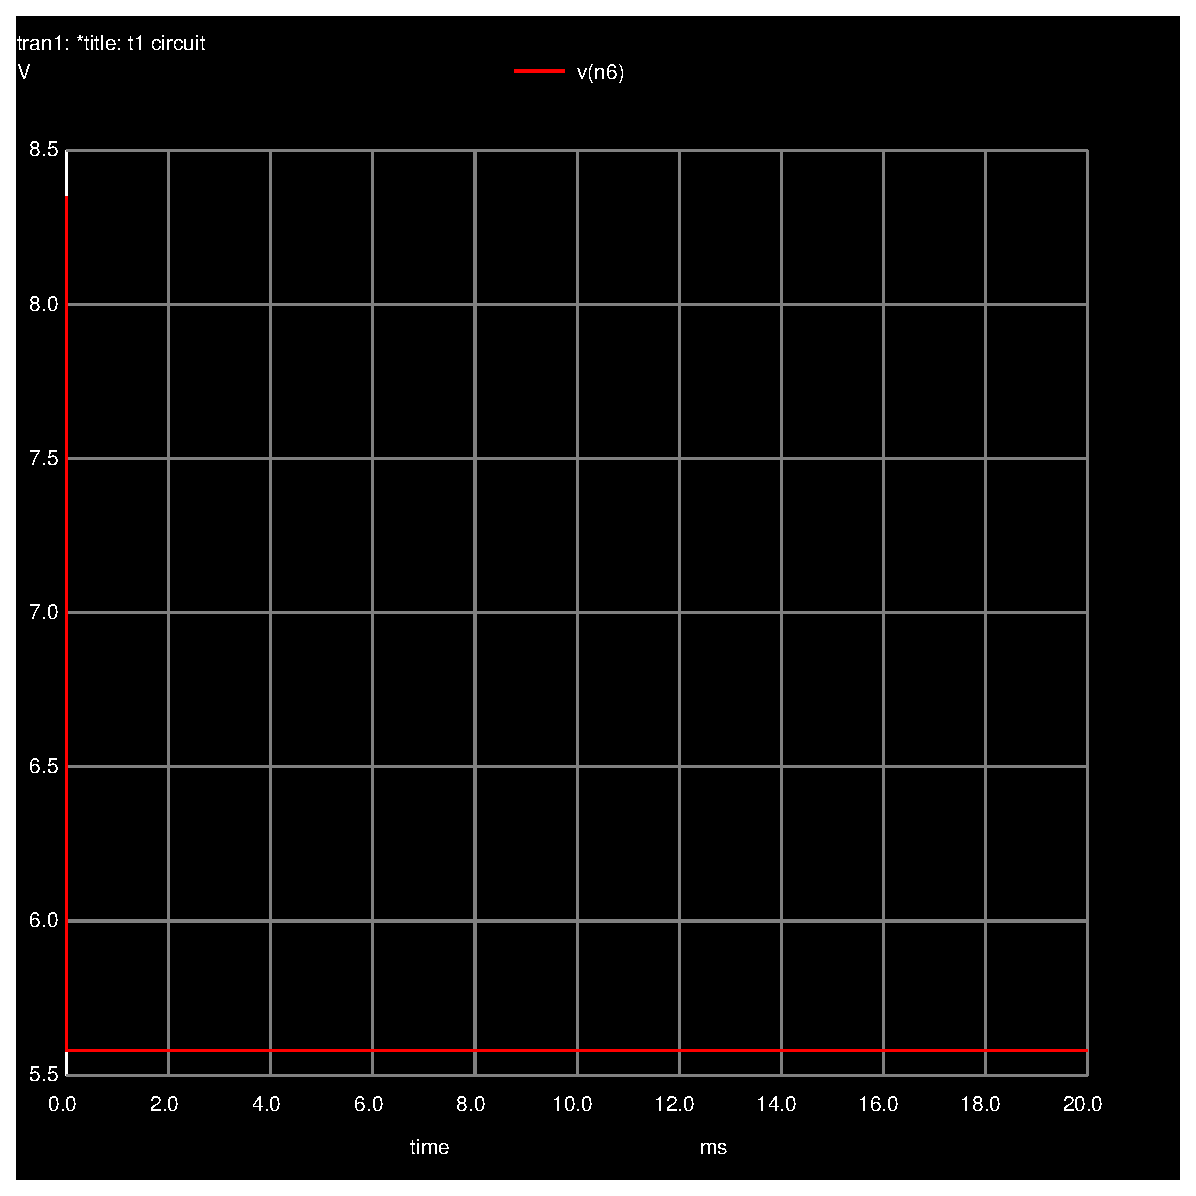
\includegraphics[width=0.8\linewidth]{trans1.ps}
%\caption{LALALAALALALALALALAL.}
%\label{fig:LALALAAL}
%\end{figure}


 %%%%%%%%%%%%%%%%%%%%%%%%%%%%%%%%%
 
\subsection{Theoretical - Topic IV}
\label{subsec:fourth_topic}

\begin{center}
   \begin{tabular}{|c||c|}
      \hline    
      \multicolumn{2}{|c|} {\bf Nodal Analysis Voltages [in Volts]} \\
      \hline
        
 Phasor of Node 1 & 6.12323399574e-17+i1.57079632679e+00 \\ \hline 
 Phasor of Node 2 & 5.78536935465e-17+i1.57079632679e+00 \\ \hline 
 Phasor of Node 3 & 5.10414916043e-17+i1.57079632679e+00 \\ \hline 
 Phasor of Node 5 & 5.83210704339e-17+i1.57079632679e+00 \\ \hline 
 Phasor of Node 6 & 8.26523333807e-02+i-1.42082340747e+00 \\ \hline 
 Phasor of Node 7 & -2.29152014669e-17+i-1.57079632679e+00 \\ \hline 
 Phasor of Node 8 & -3.40788140178e-17+i-1.57079632679e+00 \\ \hline 
   \end{tabular}
 \end{center}
 
 \paragraph
 FALTA AQUI UMA TABELA COM AS AMPLITUDES!
 
\begin{figure}[h] \centering
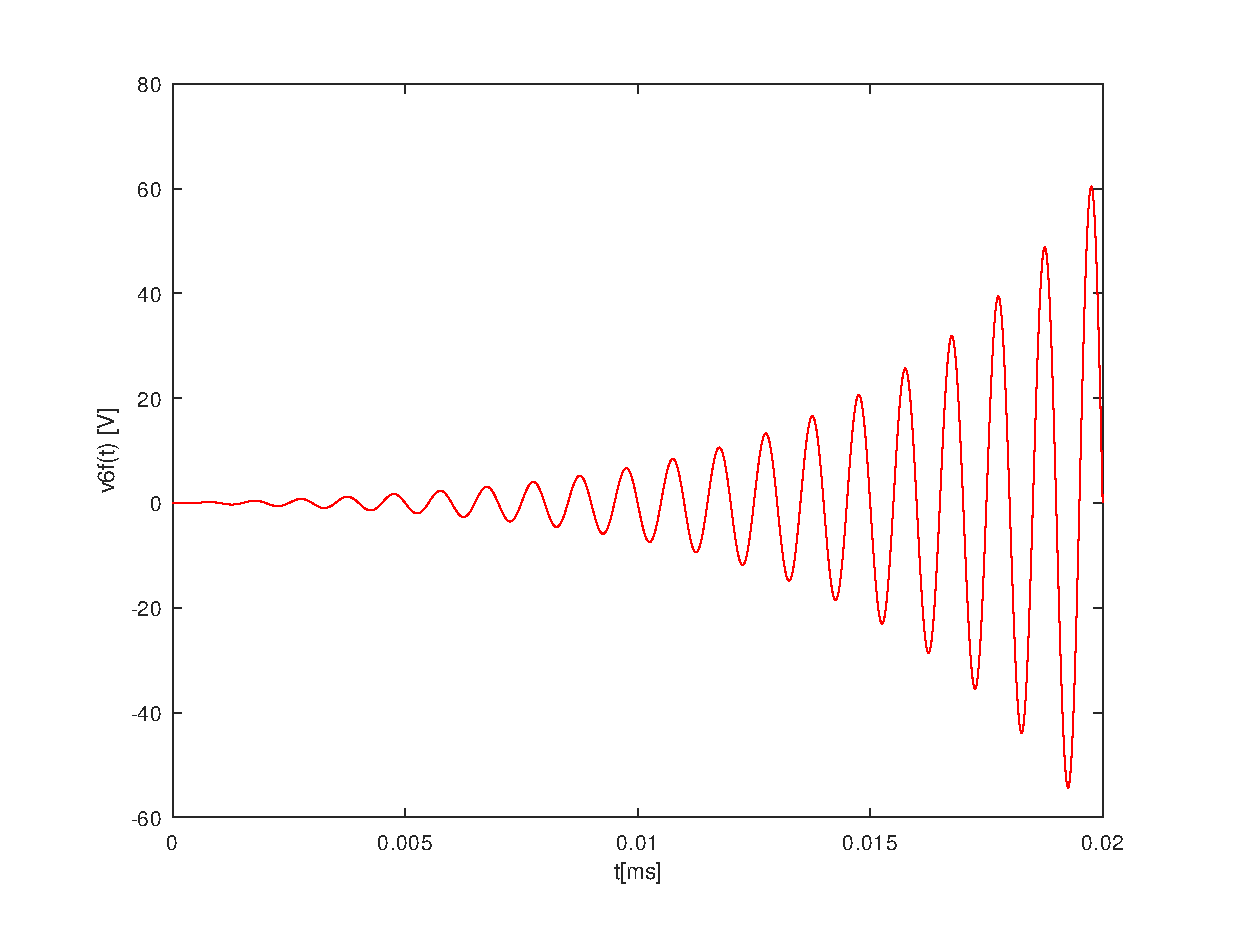
\includegraphics[width=0.8\linewidth]{forced.eps}
\caption{LALALAALALALALALALAL.}
\label{fig:LALALAAL}
\end{figure}
 
  %%%%%%%%%%%%%%%%%%%%%%%%%%%%%%%%%
 
\subsection{Theoretical - Topic V}
\label{subsec:fifth_topic}

\begin{figure}[h!] \centering
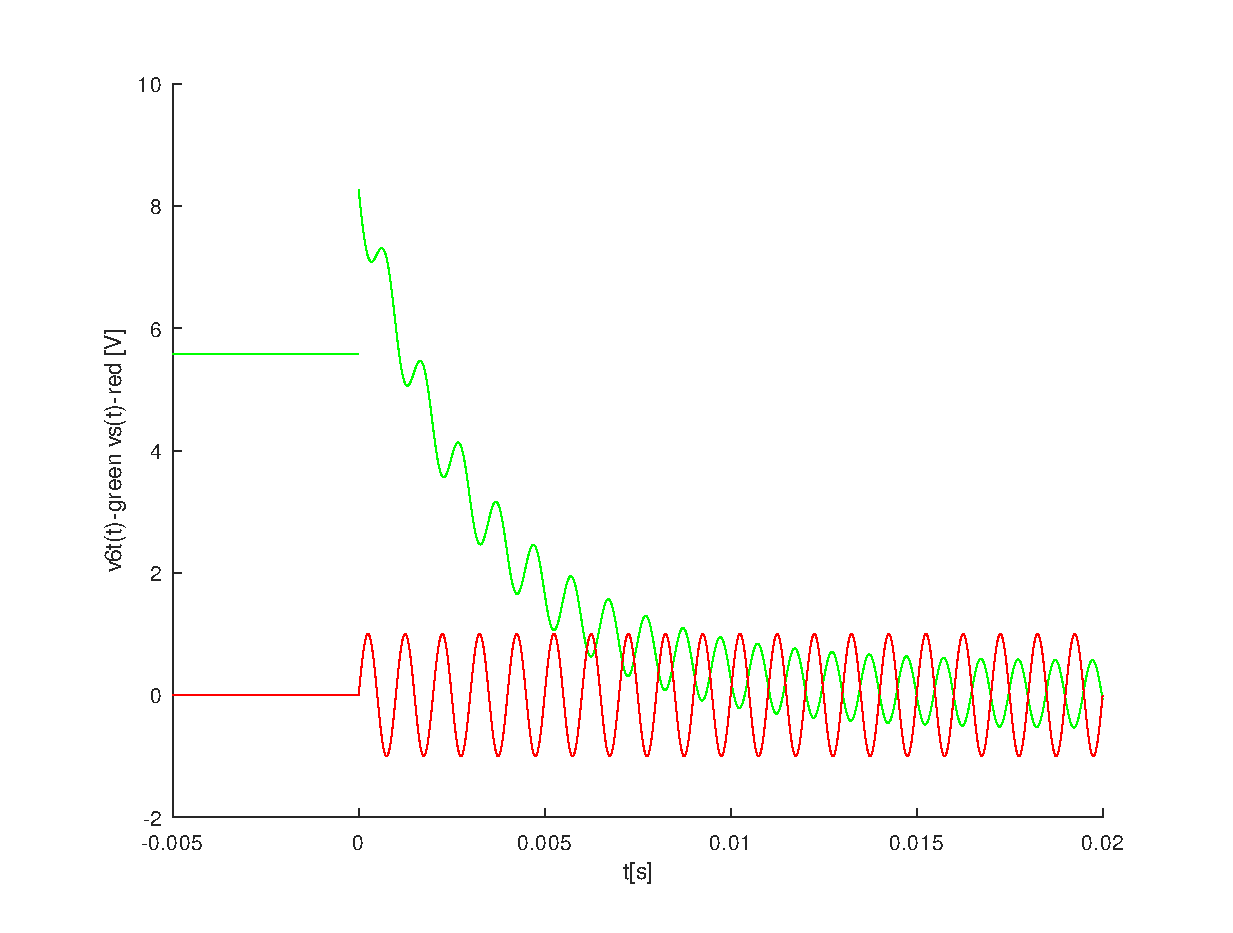
\includegraphics[width=0.8\linewidth]{total.eps}
\caption{LALALAALALALALALALAL.}
\label{fig:LALALAAL}
\end{figure}

FALTA AQUI MUITA COISA . RUI??? GRAVASTE A VERSÃO NALGUM LADO?





